\documentclass[12pt]{article}
\usepackage{tree-dvips}
\usepackage{lingmacros}
\usepackage[utf8]{inputenc}
\usepackage[spanish]{babel}
\usepackage{graphicx}

\begin{document}

\title{Requerimentos y diagramas de "Friends Night"}

\author{\textbf{11+1 Studios}\\Luis Lemus\\Victor Sanchez\\ Diego Lecanda\\Andre Cerdan}


\maketitle
\newpage

\section*{Indice}
\tableofcontents{}


\section{Requerimentos funcionales}
\fontsize{14}{18}\selectfont
Los requerimientos funcionales de la aplicaci�n \textbf{Friends Night} son:
\par 
\begin{enumerate}
\item Crear un perfil
\item Administrar perfil 
\item Cambiar imagen de perfil
\item Cambiar nombre del perfil 
\item Filtro de contenido por edad
\item Preferencias de generos de pelicula 
\item Enviar queja o comentario al soporte t�cnico
\item Ajustar el rendimiento en el dispositivo
\item Editar el perfil
\item Buscar juegos por categor�as
\item Elegir un juego
\item Jugar el juego
\item Acceder al menu de opciones
\item Regresar al menu principal 
\end{enumerate}

%nota mental: puedo poner espacios con \bigskip o con \vspace{1cm} ...  \bigskip es ir�nicamente m�s peque�o
\vspace{1cm}
\section{Requerimentos no funcionales}
\fontsize{14}{18}\selectfont
\par 
\subsection{Requerimentos de usabilidad: }
\begin{enumerate}
\item Interfaz clara que permita ver donde hay ajustes y donde es para jugar (sobre todo para usuarios no acostumbrados a la tecnolog�a);
\end{enumerate}

\subsection{Requerimentos de desarrollo: }
\begin{enumerate}
\item Trabajar con sistemas operativos de window 10 o mayor (Abstenerse de usar sistemas IOS). 
\item Las imagenes solo se podran cambiar entre las predeterminadas, no subir ninguna mas
\end{enumerate}

\subsection{Requerimentos de entorno/de software: }
\begin{enumerate}
\item Sistemas IOs y Android

\end{enumerate}

\subsection{Requerimentos de eficiencia: }
\begin{enumerate}
\item La aplicaci�n no debe tardar mucho tiempo en conectar a los jugadores entre ellos.
\end{enumerate}

\subsection{Requerimentos de disponibilidad: }
\begin{enumerate}
\item Mostrar desde el �rea de descarga la compatibilidad con dispositivos Android e IOS
\end{enumerate}

\subsection{Requerimentos de mantenimiento: }
\begin{enumerate}
\item Version de unity 2021.3.8f LTS con mantenimiento de 3 a�os desde que sali� 
\end{enumerate}

\subsection{Requerimentos regulatorios: }
\begin{enumerate}
\item Acatar regulaciones respecto a contenido +18 respecto a consumo de alcohol 
\end{enumerate}

\subsection{Requerimentos eticos }
\begin{enumerate}
\item Advertir acerca de los juegos +18 de bebida, tanto en la p�gina donde se publique el juego como dentro del juego
\end{enumerate}

%%%%%%%%%%%%%%%%%%55

\section{Diagrama de casos de uso}

\begin{figure}[h]
    \begin{flushleft}
        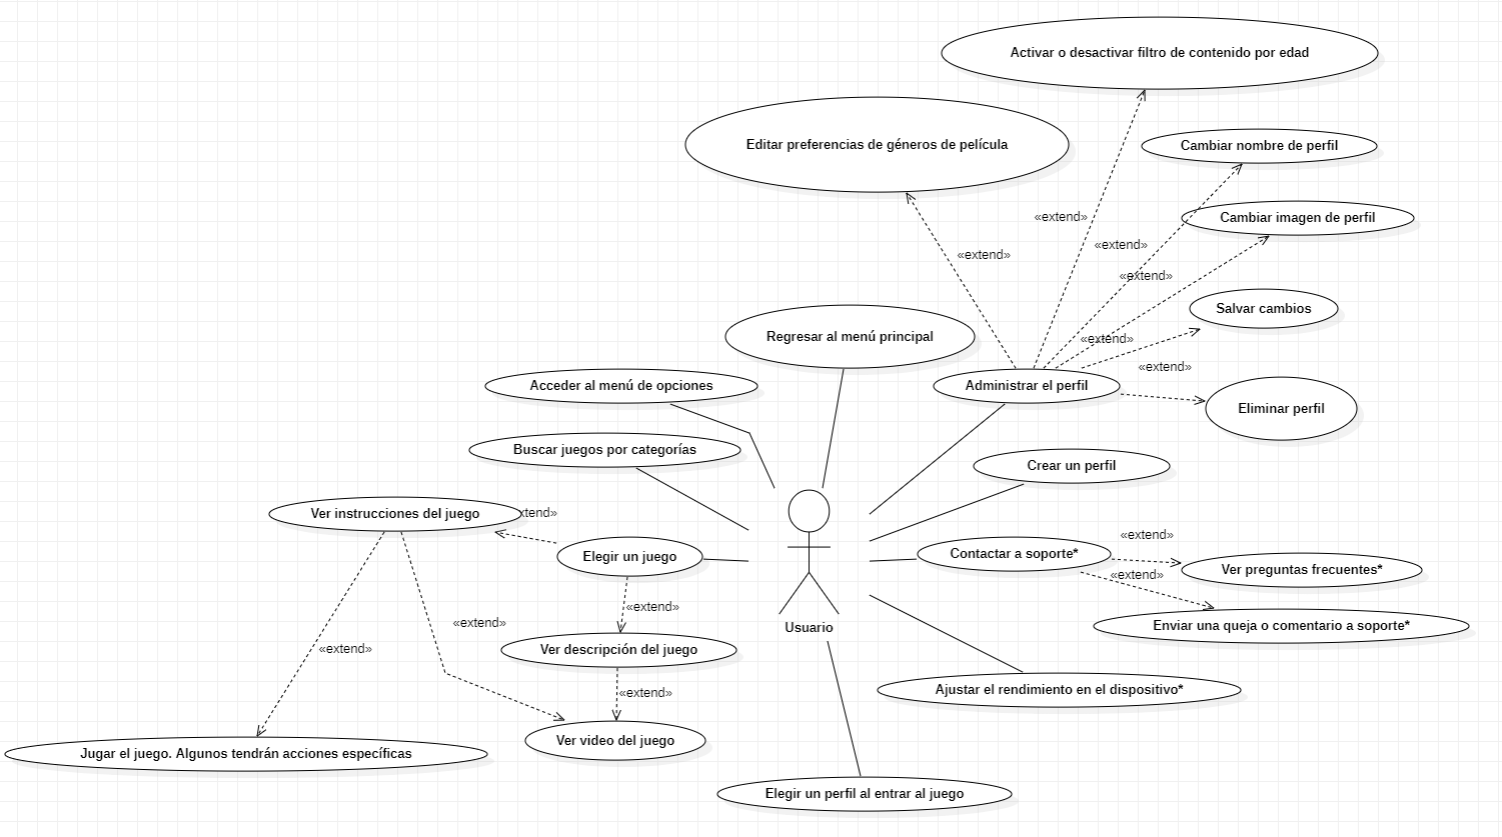
\includegraphics[width=1.3\textwidth]{DiagramaUsoDeCasoFN.png}
        \caption{Diagrama de uso de caso}
        \label{Diagrama}
    \end{flushleft}
\end{figure}


\vspace{1cm}
%%%%%%%%%%%%%%%%%%%%%%%%%%%%%%%%%%%%%%%%%%%%%%%
\section{Diagrama de entidad relacion }
\fontsize{14}{18}\selectfont
\par 
El siguiente diagrama de entidad relacion de \textbf{Friends Night} contempla las distintas tablas que tendra la base de datos para guardar informacion:

\begin{center}
	\centering
		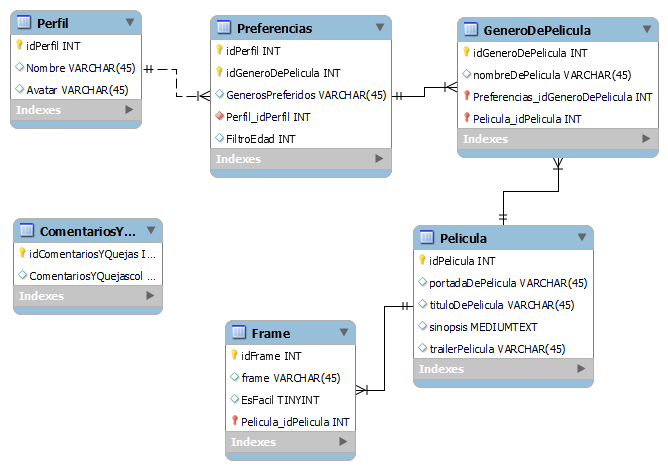
\includegraphics[width=1.2\textwidth]{DiagramaEntidadRelacionFriendsNight.png}

	\caption{Diagrama de entidad relacion}
	\label{DiagramaER}
\end{center}
\vspace{1cm}
%%%%%%%%%%%%%%%%%%%%%%%%%%%%%%
\section{Diagrama de componentes}
\fontsize{14}{18}\selectfont
\par 
El siguiente diagrama de componentes de \textbf{Friends Night} contempla la arquitectura con la que se conectaran la base de datos, el juego y el usuario

\begin{center}
	\centering
		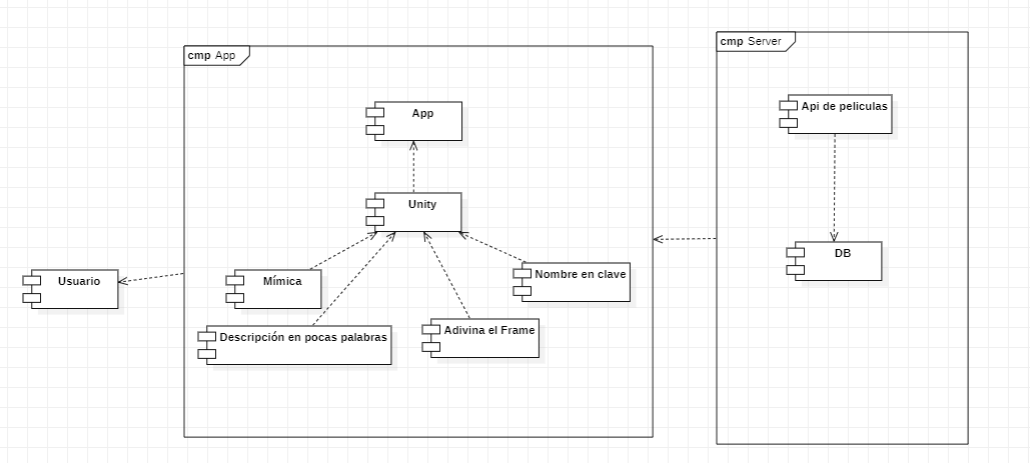
\includegraphics[width=1.2\textwidth]{DiagramaDeComponentesFriendsNight.png}

	\caption{Diagrama de componentes}
	\label{DiagramaComponentes}
\end{center}
\vspace{1cm}
%%%%%%%%%%%%%%%%%%%%%%%%%

\section{Diagrama de clases }
\fontsize{14}{18}\selectfont
\par 
El siguiente diagrama de clases de \textbf{Friends Night} contempla las distintas clases que se programaran en el desarrollo del juego:

\begin{center}
	\centering
		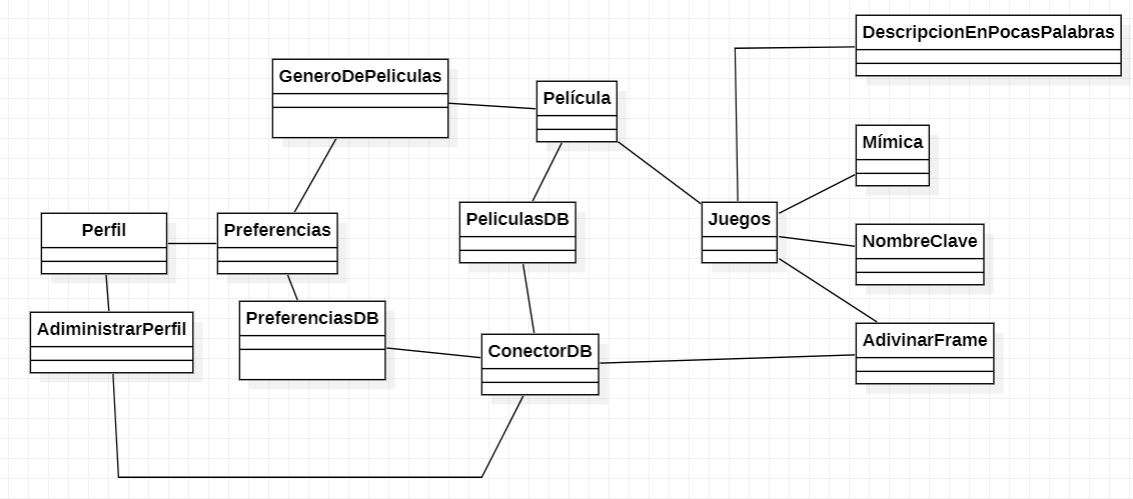
\includegraphics[width=1.2\textwidth]{DiagramaDeClasesFriendsNight.png}

	\caption{Diagrama de clases}
	\label{DiagramaClases}
\end{center}
\vspace{1cm}
%nota mental: puedo poner espacios con \bigskip o con \vspace{1cm} ...  \bigskip es ir�nicamente m�s peque�o
%%%%%%%%%%%%%%%%%%%%%%%%%%%%%%
\section{Diagramas de secuencia:}
\fontsize{14}{18}\selectfont
\par 
A continuacion van los diagramas de secuencia para los distintos casos de uso.

El primero refiere al caso de buscar un juego:

\begin{center}
	\centering
		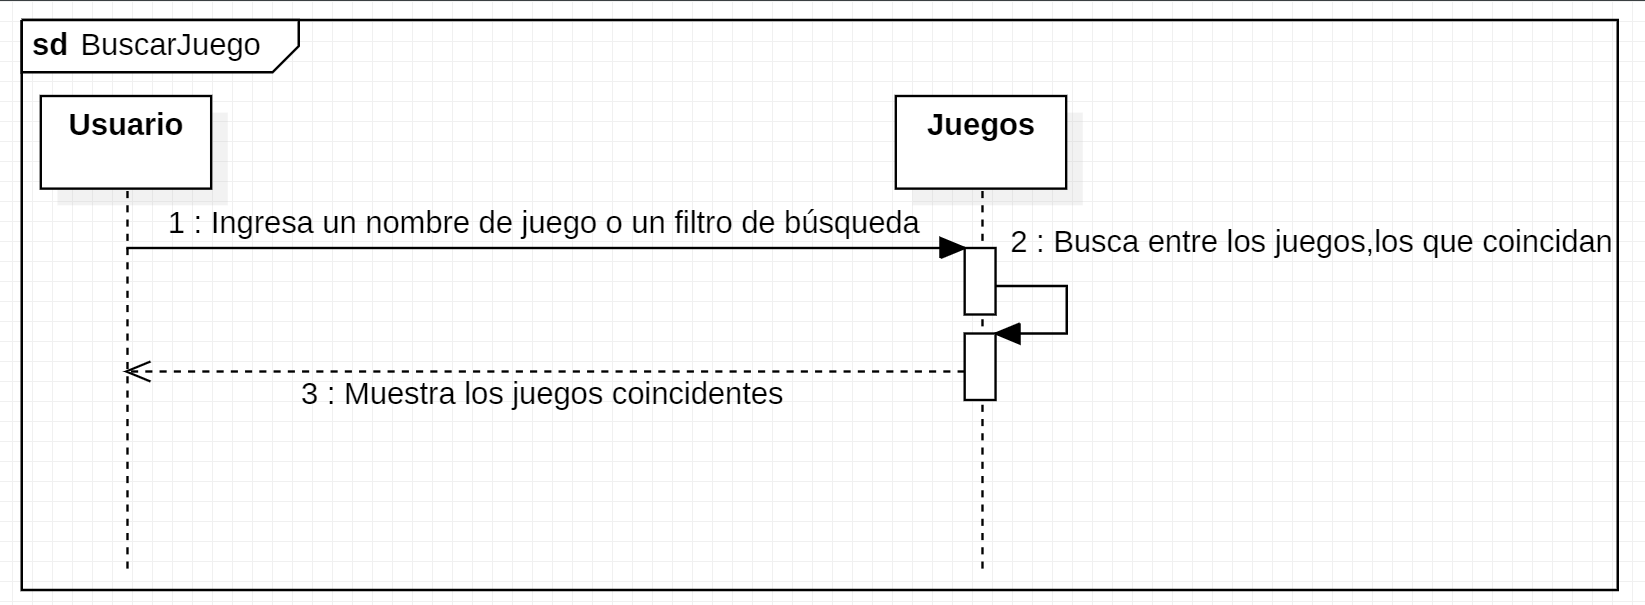
\includegraphics[width=1.2\textwidth]{DSFNBuscarJuego.png}

	\caption{Diagrama de secuencia para buscar un juego}
	\label{DSFNBuscarJuego}
\end{center}

\begin{center}
	\centering
		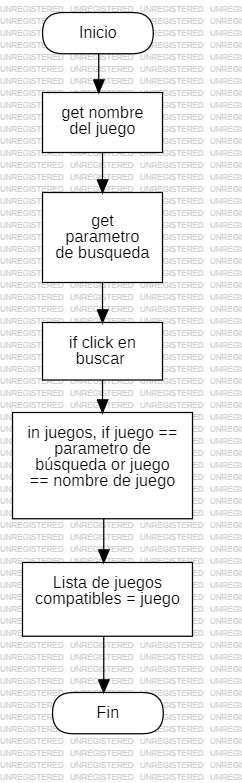
\includegraphics[width=0.4\textwidth]{DFFNBuscarJuego.jpg}

	\caption{Diagrama de flujo para buscar un juego}
	\label{DFFNBuscarJuego}
\end{center}
%%%%%%%%%%%%%%%%%%%%%
\bigskip
\fontsize{14}{18}\selectfont
\par 
En el segundo diagrama se plasma como seria la creacion y edicion de un nuevo perfil:

\begin{figure}[h]
    \begin{flushleft}
        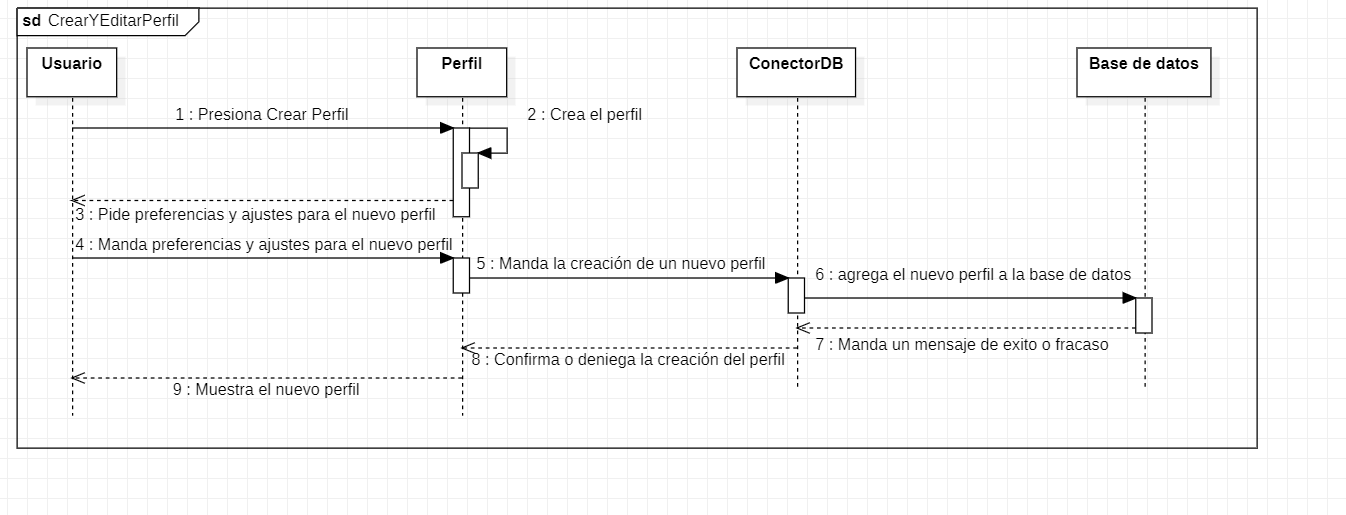
\includegraphics[width=1.3\textwidth]{DSFNCrearYEditarPerfil.png}
        \caption{Diagrama de secuencia para crear y editar un perfil nuevo}
        \label{DSFNCrearYEditarPerfil}
    \end{flushleft}
\end{figure}


\begin{center}
	\centering
		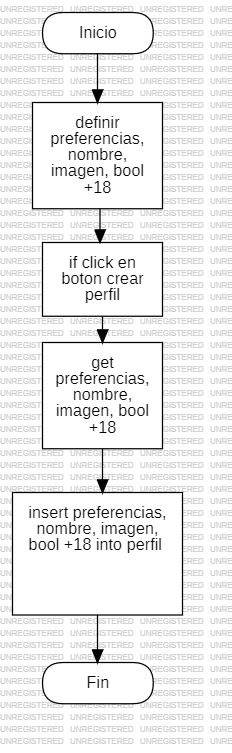
\includegraphics[width=0.4\textwidth]{DFFNCrearYEditarPerfil.jpg}

	\caption{Diagrama de flujo para crear y editar un perfil nuevo}
	\label{DFFNCrearYEditarPerfil}
\end{center}

\bigskip
%%%%%%%%%%%%%%%%%%%%%%%
\fontsize{14}{18}\selectfont
\par 
En el tercer diagrama propone la secuencia para la edicion de la informacion o preferencias de un perfil ya existente:

\begin{figure}[h]
    \begin{flushleft}
        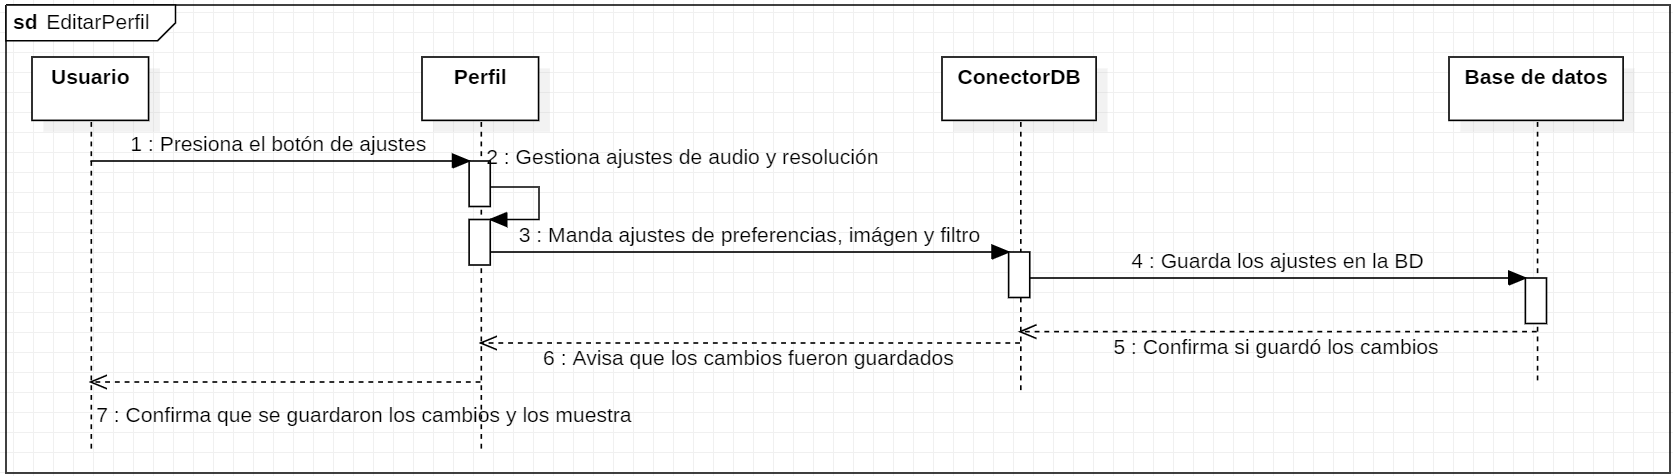
\includegraphics[width=1.2\textwidth]{DSFNEditarPerfil.png}
        \caption{Diagrama de secuencia para editar un perfil ya existente}
        \label{DSFNEditarPerfil}
    \end{flushleft}
\end{figure}


\begin{center}
	\centering
		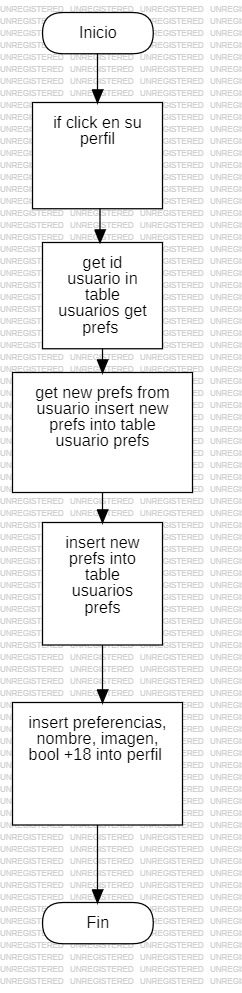
\includegraphics[width=0.3\textwidth]{DFFNEditarPerfil.jpg}

	\caption{Diagrama de flujo para editar un perfil ya existente}
	\label{DFFNEditarPerfil}
\end{center}

\bigskip

%%%%%%%%%%%%%%%%%%%%%%%
\fontsize{14}{18}\selectfont
\par 
El cuarto diagrama plantea la eleccion de un juego:

\begin{figure}[h]
    \begin{flushleft}
        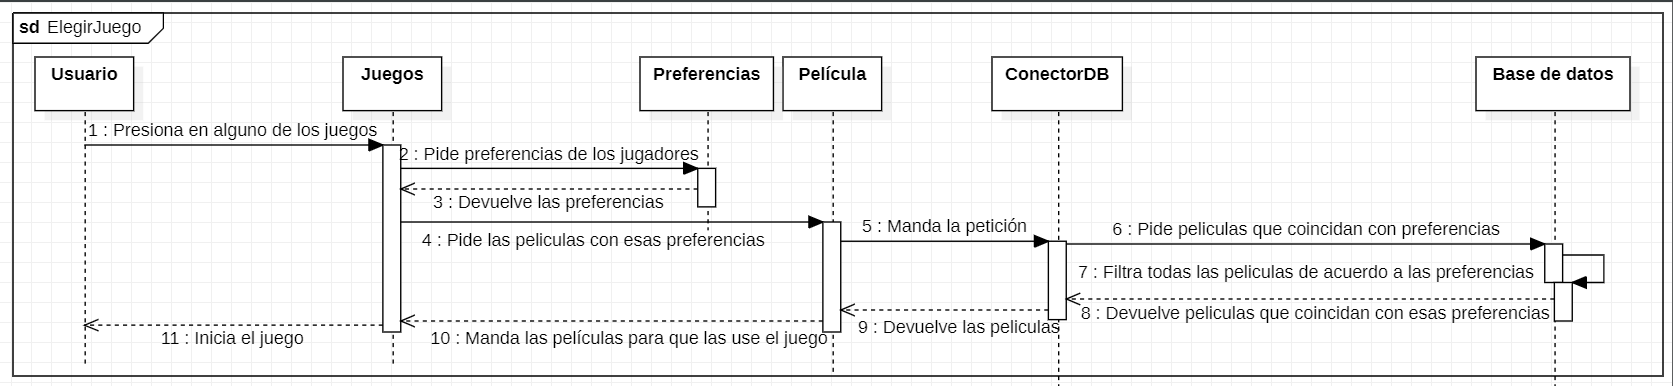
\includegraphics[width=1.3\textwidth]{DSFNElegirJuego.png}
        \caption{Diagrama de secuencia para elegir un juego}
        \label{DSFNElegirJuego}
    \end{flushleft}
\end{figure}


\begin{center}
	\centering
		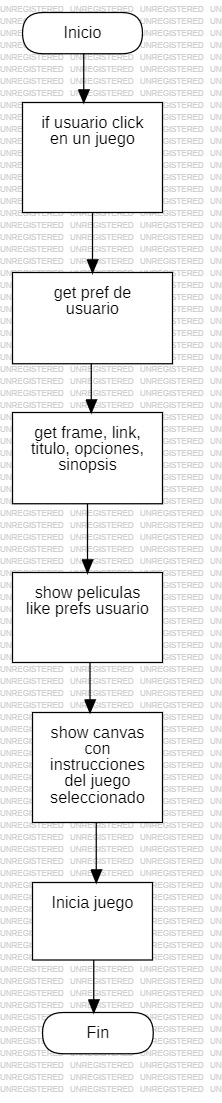
\includegraphics[width=0.2\textwidth]{DFFNElegirJuego.jpg}

	\caption{Diagrama de flujo para elegir un juego}
	\label{DFFNElegirJuego}
\end{center}

\bigskip
%%%%%%%%%%%%%%%%%
\fontsize{14}{18}\selectfont
\par 
El quinto diagrama propone la secuencia para cambiar las opciones de la interfaz de configuracion:

\begin{center}
	\centering
		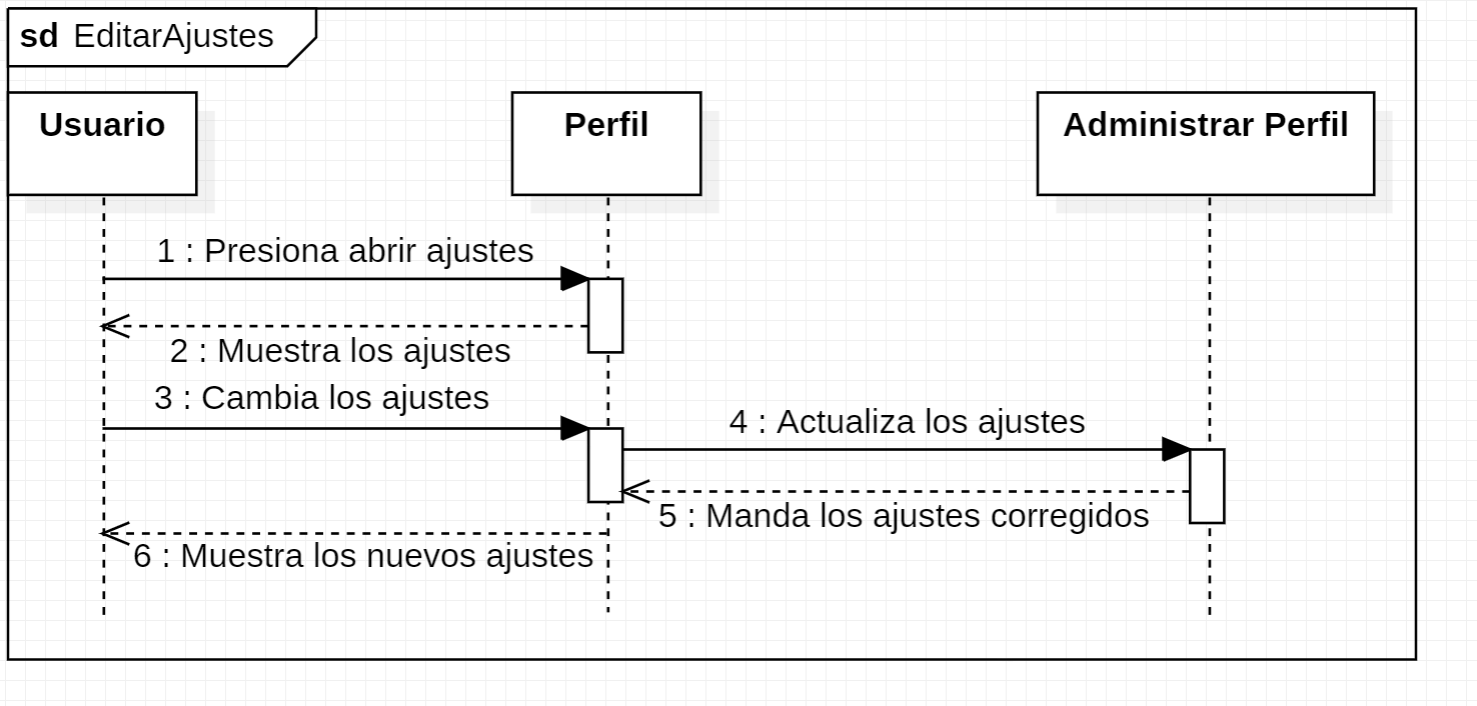
\includegraphics[width=1\textwidth]{DSFNEditarAjustes.png}

	\caption{Diagrama de secuencia para editar las opciones en configuracion}
	\label{DSFNopcionesConfig}
\end{center}

\begin{center}
	\centering
		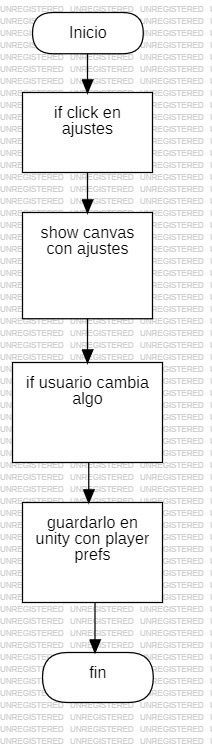
\includegraphics[width=0.4\textwidth]{DFFNEditarAjustes.jpeg}

	\caption{Diagrama de flujo para editar las opciones en configuracion}
	\label{DFFNopcionesConfig}
\end{center}

\bigskip
%%%%%%%%%%%%%%%%%%%%%%
\fontsize{14}{18}\selectfont
\par 
En el sexto diagrama se propone la secuencia para regresar al menu principal:

\begin{center}
	\centering
		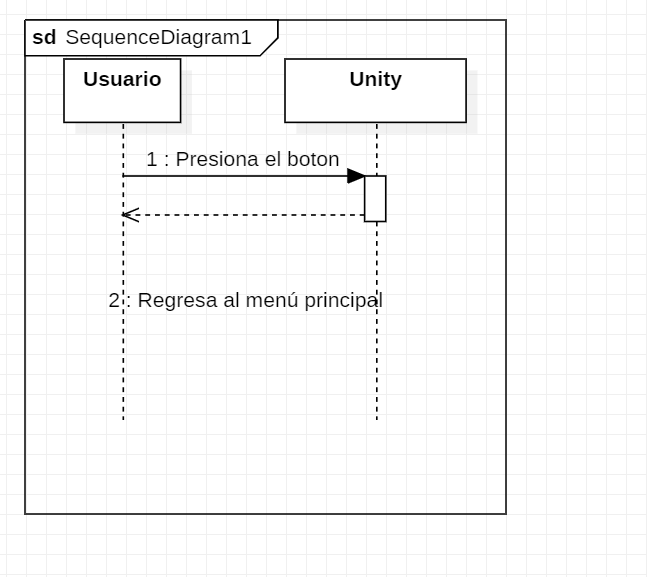
\includegraphics[width=0.9\textwidth]{DSFNRegresarAMenu.png}

	\caption{Diagrama de secuencia para regresar al menu principal}
	\label{DSFNRegresarAMenu}
\end{center}


\begin{center}
	\centering
		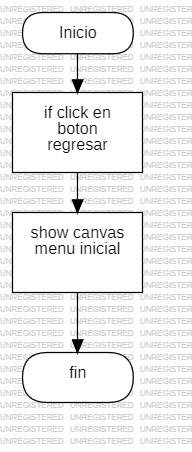
\includegraphics[width=0.4\textwidth]{DFFNRegresarAMenu.jpeg}

	\caption{Diagrama de flujo para regresar al menu principal}
	\label{DFFNRegresarAMenu}
\end{center}


\bigskip
%%%%%%%%%%%%%%%55
\fontsize{14}{18}\selectfont
\par 
Para el septimo diagrama plantea el contacto a soporte, sin embargo, esta opcion dependera del tiempo de desarrollo de la aplicacion:

\begin{figure}[h]
    \begin{flushleft}
        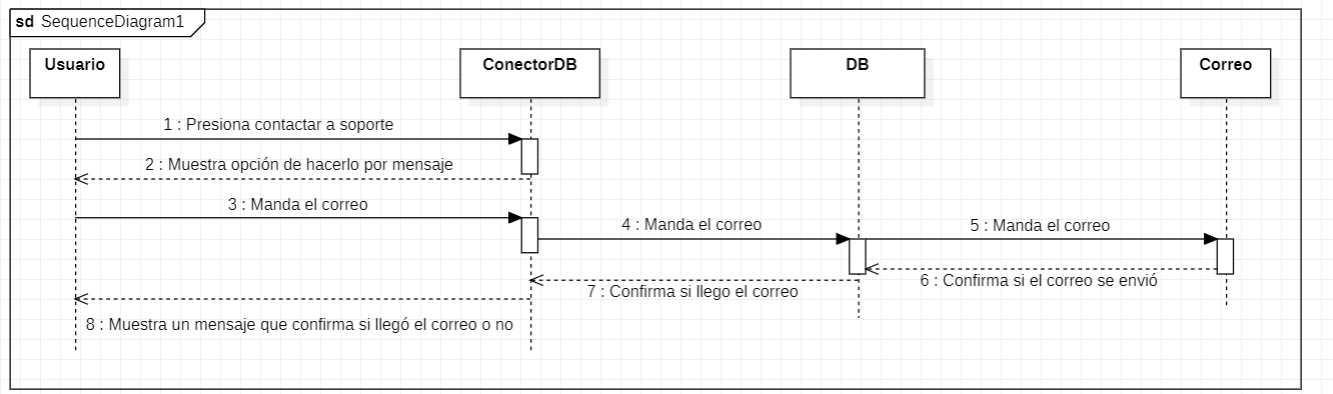
\includegraphics[width=1.3\textwidth]{DSFNContactarSoporte.png}
        \caption{Diagrama de secuencia para contactar a soporte}
        \label{DSFNContactoSoporte}
    \end{flushleft}
\end{figure}


	\centering
		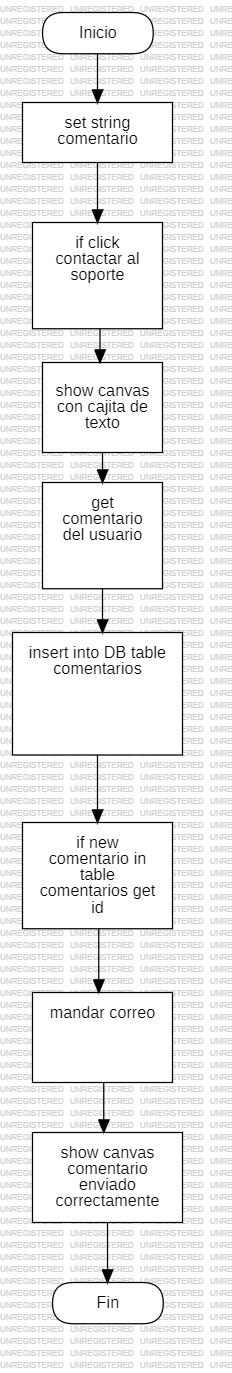
\includegraphics[width=0.2\textwidth]{DFFNContactarSoporte.jpg}

	\caption{Diagrama de flujo para contactar a soporte}
	\label{DFFNContactoSoporte}
\end{center}


%%%%%%%%%%%%%%%%
\bigskip
\fontsize{14}{18}\selectfont
\par 
En el octavo diagrama se propone la secuencia para jugar el juego de Adivina Frame  y el diagrama de flujo respectivo:

\begin{center}
	\centering
		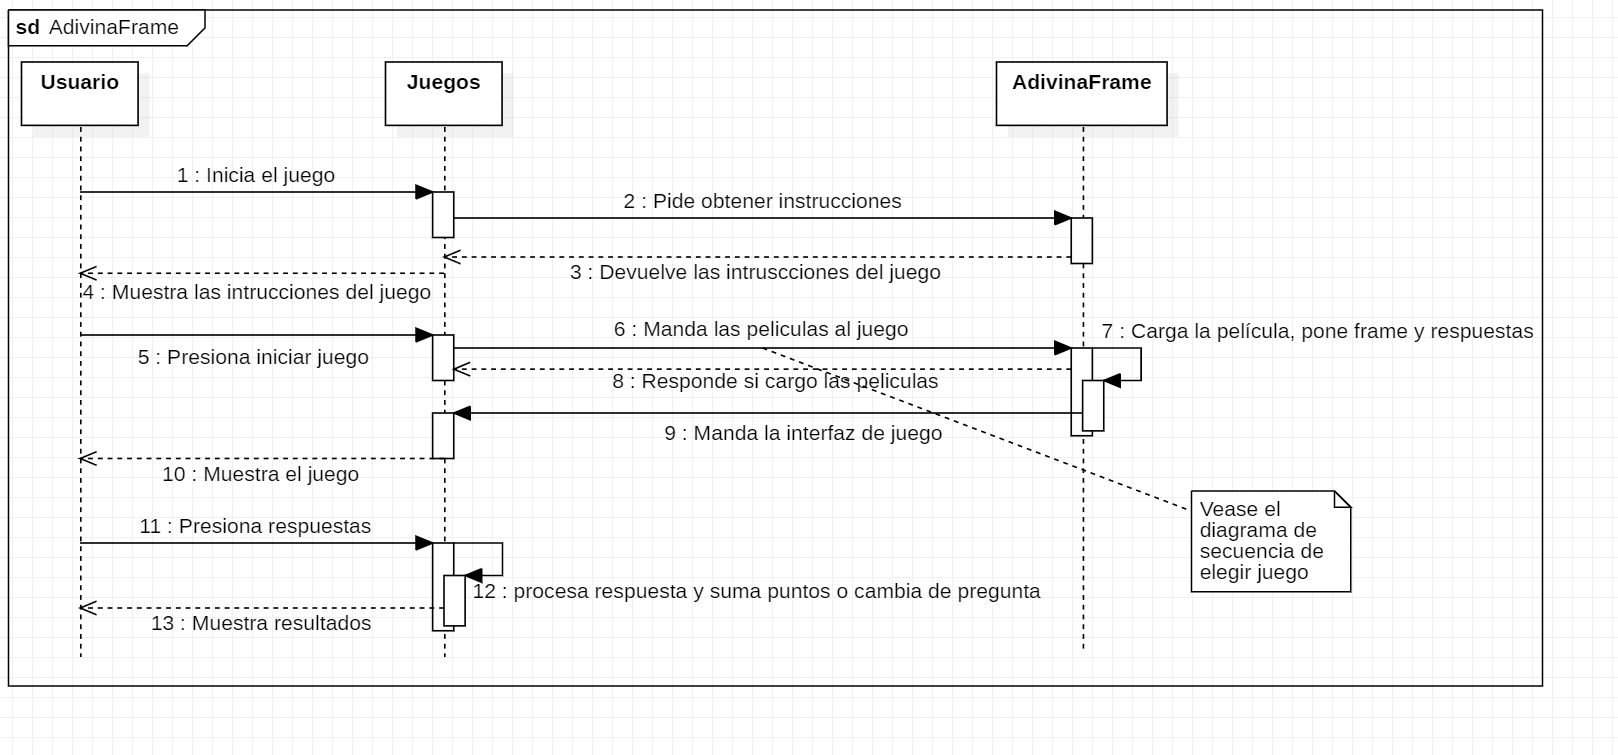
\includegraphics[width=1.3\textwidth]{DSFNAdvinaFrame.png}

	\caption{Diagrama de secuencia para jugar Adivina Frame}
	\label{DSFNAdivinaFrame}
\end{center}

\begin{center}
	\centering
		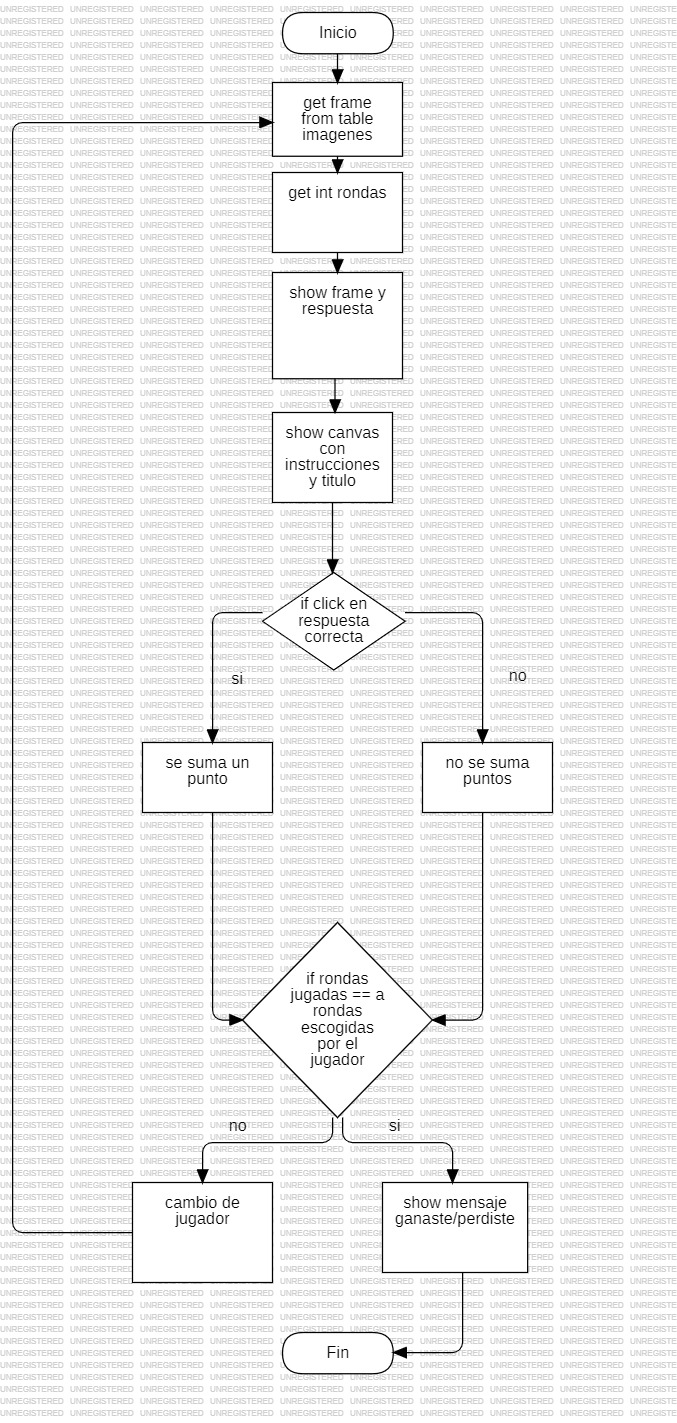
\includegraphics[width=0.7\textwidth]{DFFNAdvinaFrame.jpg}

	\caption{Diagrama de flujo para jugar Adivina Frame}
	\label{DFFNAdivinaFrame}
\end{center}
%%%%%%%%%%%%%%%%%%%%%%%%5
\bigskip
\fontsize{14}{18}\selectfont
\par 
En el noveno diagrama se propone la secuencia para jugar el juego de descripcion en pocas palabras  y el diagrama de flujo respectivo:

\begin{center}
	\centering
		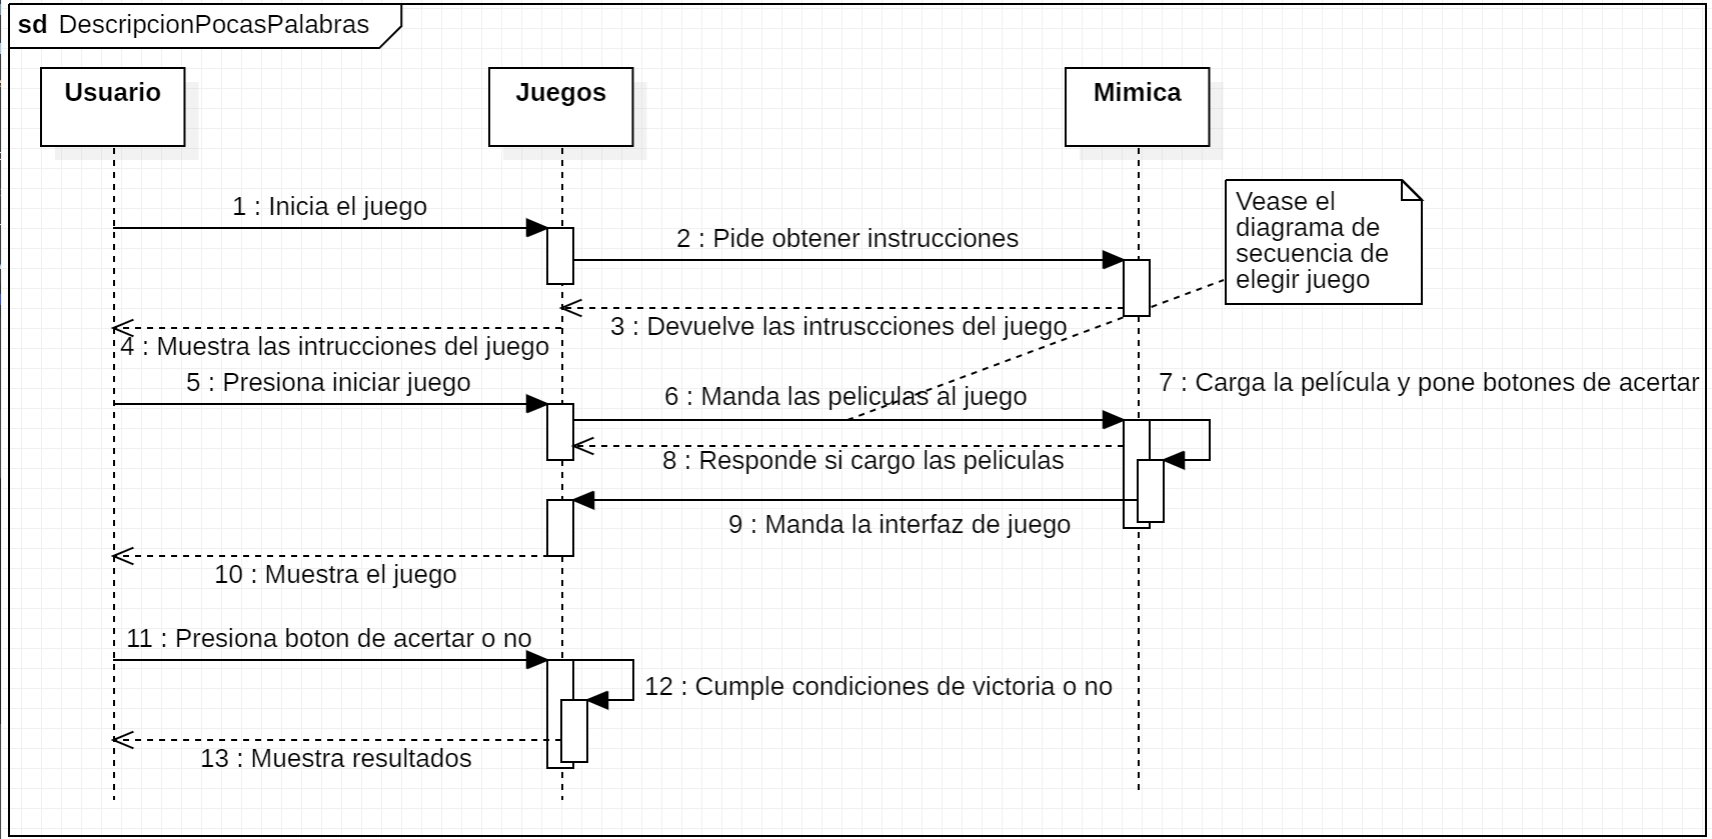
\includegraphics[width=1.29\textwidth]{DSFNDescripcionEnPocasPalabras.png}

	\caption{Diagrama de secuencia para jugar descripcion en pocas palabras}
	\label{DSFNDescric}
\end{center}
\begin{center}
	\centering
		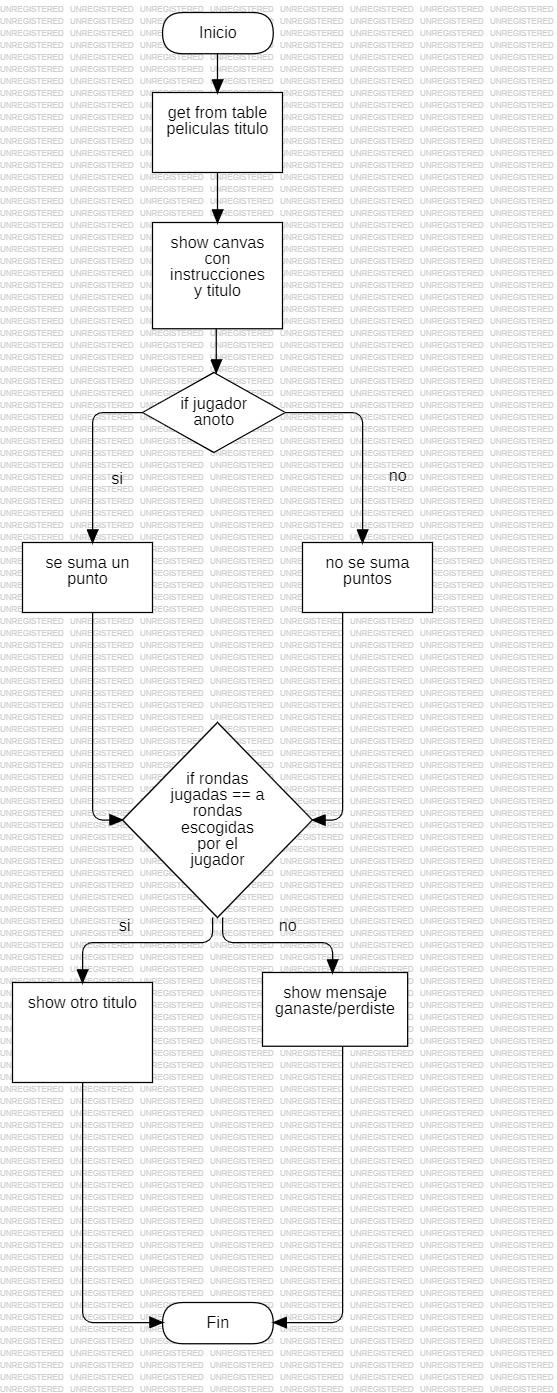
\includegraphics[width=0.56\textwidth]{DFFNDescripcionEnPocasPalabras.jpg}

	\caption{Diagrama de flujo para jugar descripcion en pocas palabras}
	\label{DFFNDescric}
\end{center}
%%%%%%%%%%%%%%%%%%%5
\bigskip
\fontsize{14}{18}\selectfont
\par 
En el decimo diagrama se propone la secuencia para jugar el juego de mimica y el diagrama de flujo respectivo:

\begin{center}
	\centering
		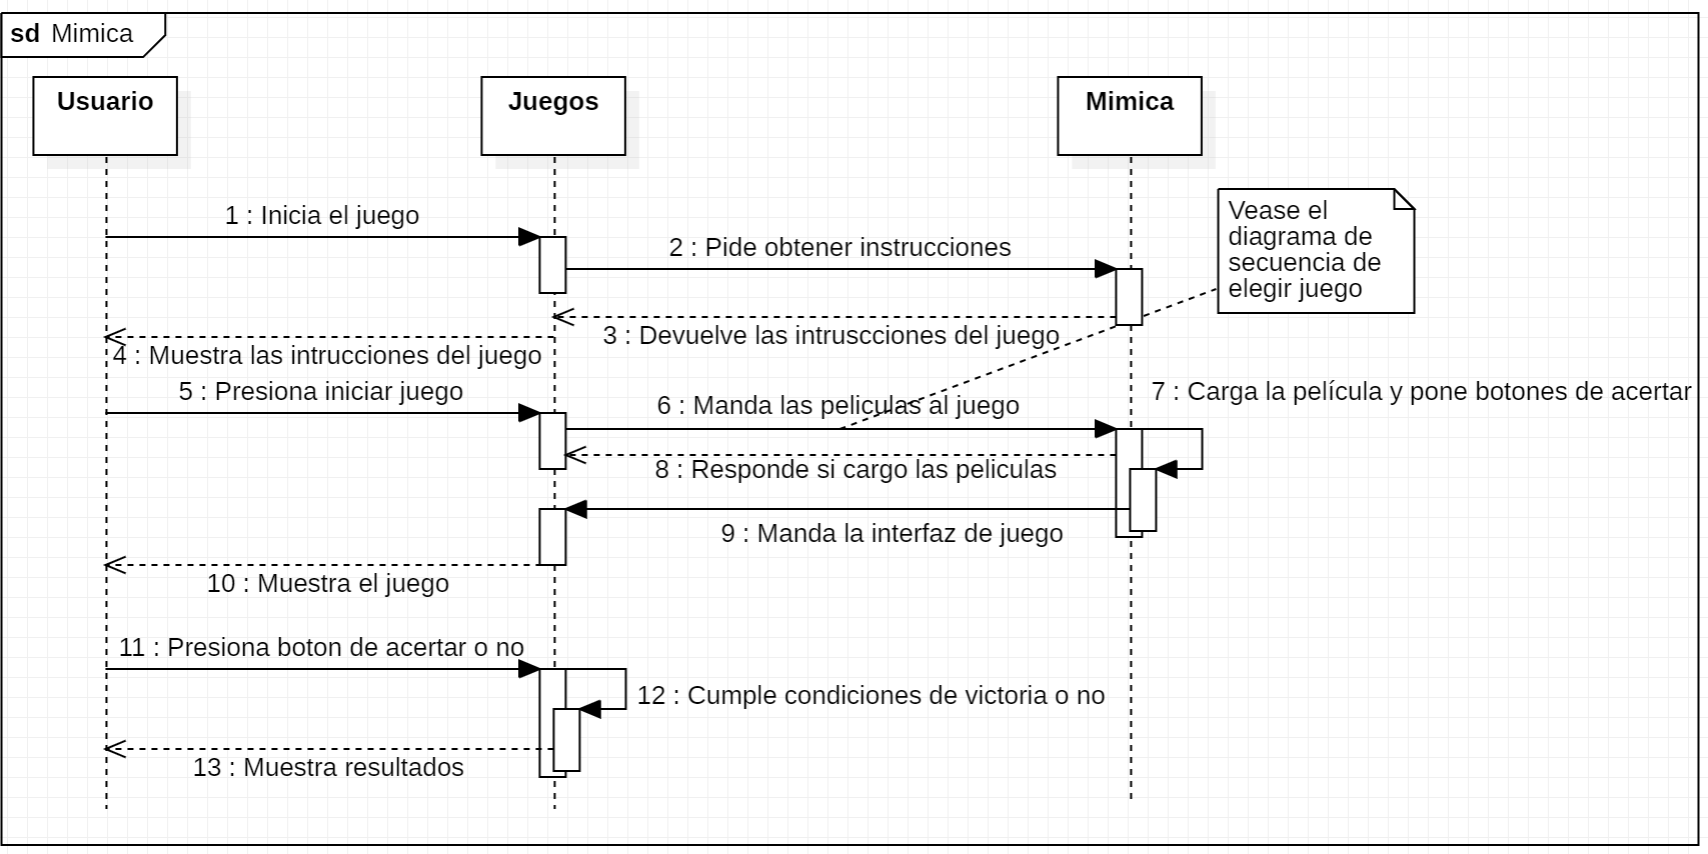
\includegraphics[width=1.29\textwidth]{DSFNMimica.png}

	\caption{Diagrama de secuencia para jugar Mimica}
	\label{DSFNMimica}
\end{center}

\begin{center}
	\centering
		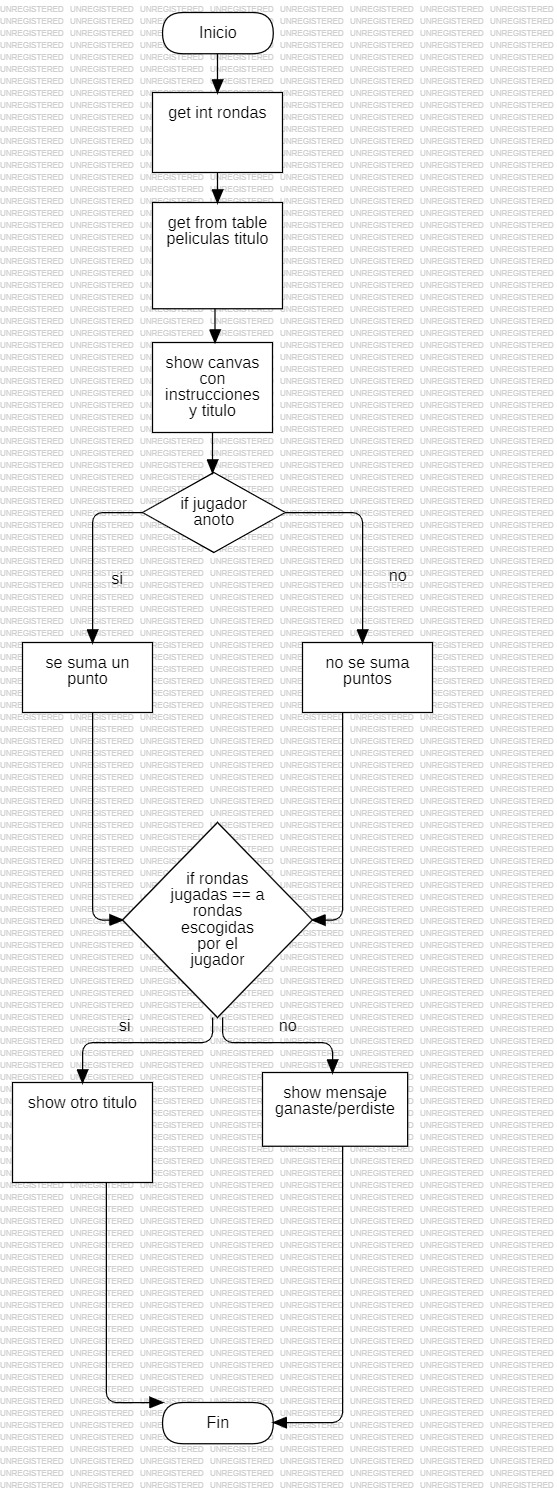
\includegraphics[width=0.5\textwidth]{DFFNMimica.jpg}

	\caption{Diagrama de flujo para jugar Mimica}
	\label{DFFNMimica}
\end{center}
%%%%%%%%%%%%%%%%%%%5
\bigskip
\fontsize{14}{18}\selectfont
\par 
En el onceavo diagrama se propone la secuencia para jugar el juego de Nombre Clave y el diagrama de flujo respectivo:

\begin{center}
	\centering
		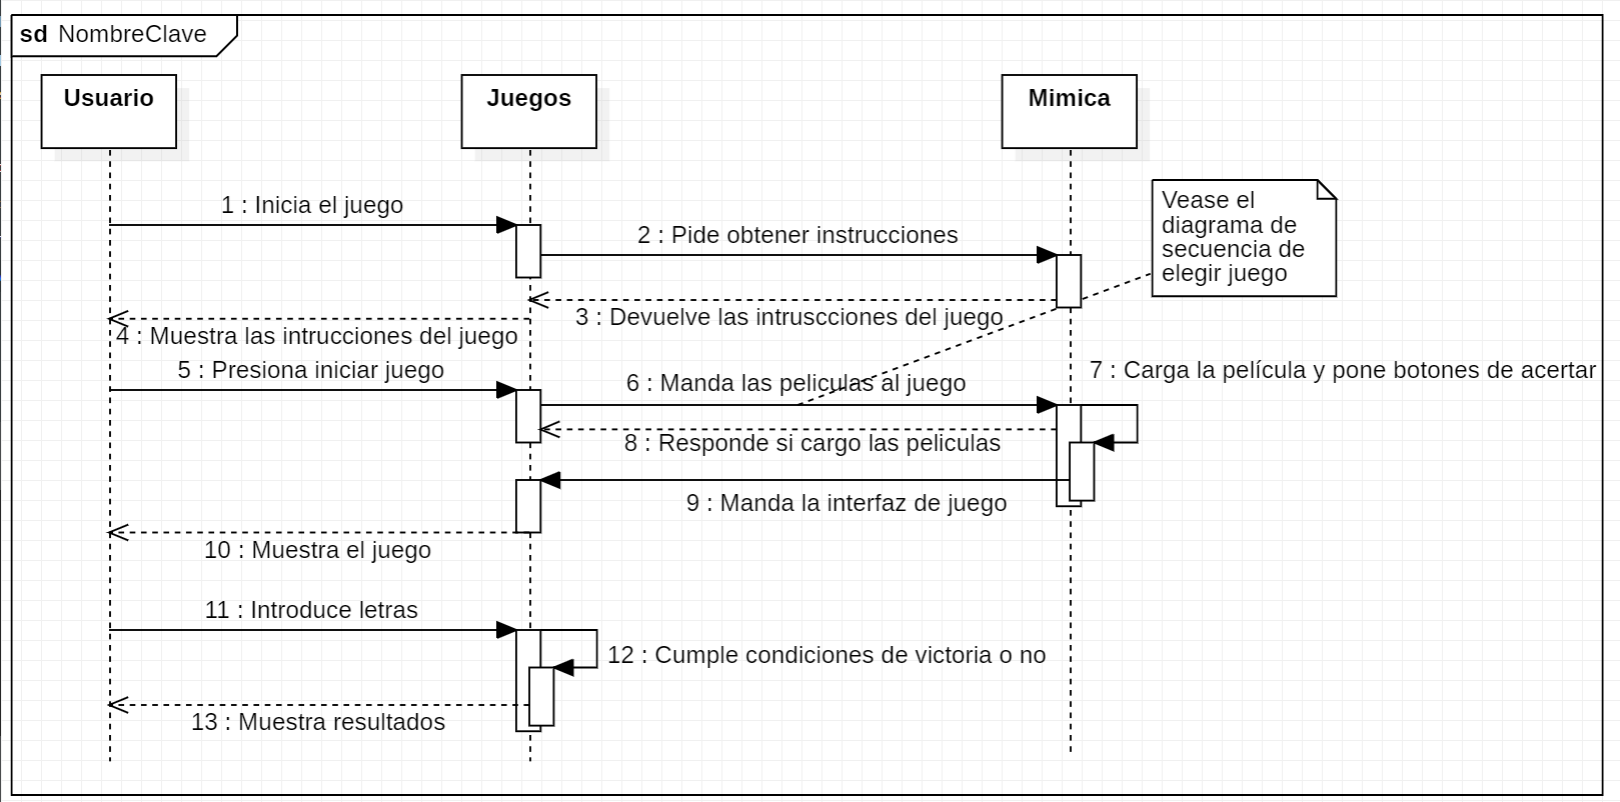
\includegraphics[width=1.29\textwidth]{DSFNNombreClave.png}

	\caption{Diagrama de secuencia para jugar Nombre Clave}
	\label{DSFNC}
\end{center}

\begin{center}
	\centering
		\includegraphics[width=0.5\textwidth]{DFFNNombreClave.jpg}

	\caption{Diagrama de flujo para jugar Nombre Clave}
	\label{DSFNC}
\end{center}


%%%%%%%%%%%%%%%%%%%5
\bigskip
\fontsize{14}{18}\selectfont
\par 
En el doceavo diagrama se propone la secuencia para elegir el perfil al iniciar el juego con su diagrama de flujo respectivo:

\begin{figure}[h]
    \begin{flushleft}
        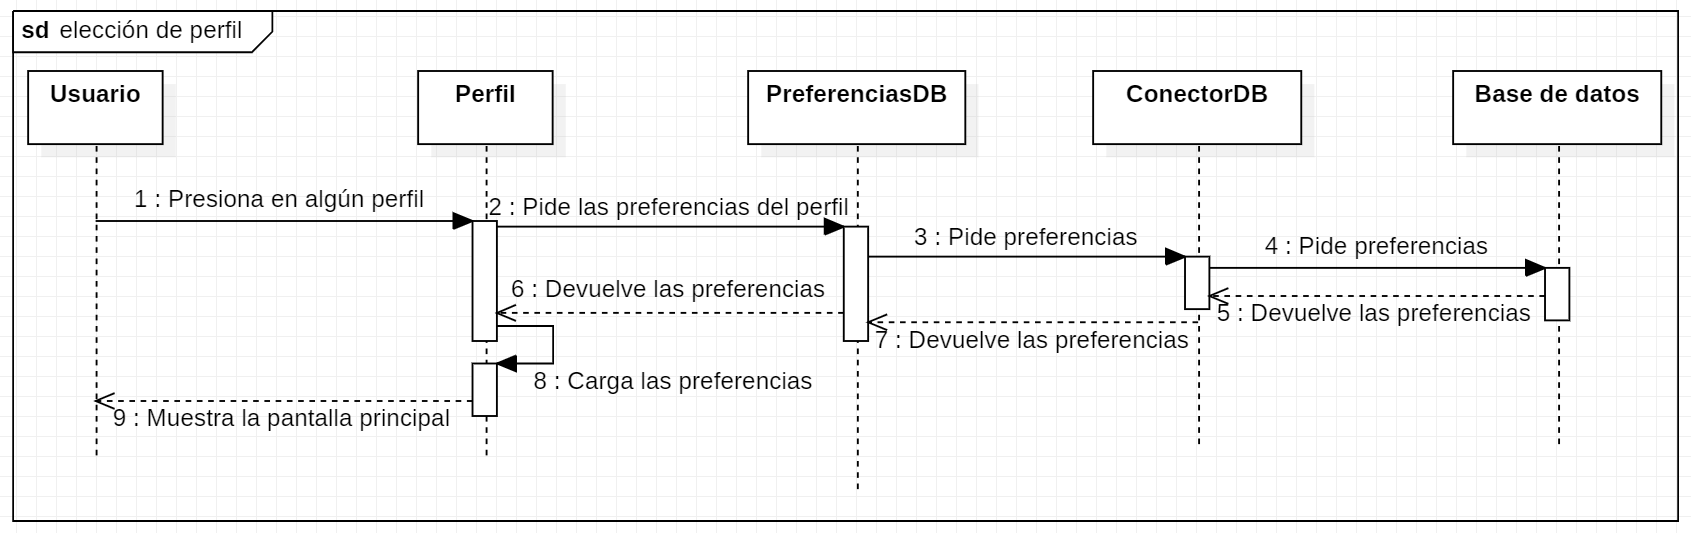
\includegraphics[width=1.3\textwidth]{DSFNElegirPerfil.png}
        \caption{Diagrama de secuencia para elegir perfil}
        \label{DSFNC}
    \end{flushleft}
\end{figure}


\begin{center}
	\centering
		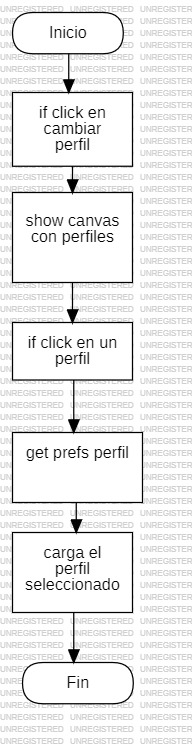
\includegraphics[width=0.3\textwidth]{DFFNEleccionPerfil.jpg}

	\caption{Diagrama de flujo para elegir el perfil}
	\label{DSFNC}
\end{center}

%%
\end{document}

